\documentclass[a4paper, 11pt]{report}

\usepackage[style=numeric]{biblatex}
\usepackage[utf8]{inputenc}
\usepackage{amsmath}
\usepackage{etoolbox}
\usepackage{float}
\usepackage{geometry}
\usepackage{graphicx}
\usepackage{hyperref}

\addbibresource{References.bib}
\graphicspath{ {images/} }

\makeatletter

\patchcmd{\@makechapterhead}{50\p@}{\chapheadtopskip}{}{}
\patchcmd{\@makeschapterhead}{50\p@}{\chapheadtopskip}{}{}

\makeatother

\newlength{\chapheadtopskip}\setlength{\chapheadtopskip}{0mm}

\title{
	{Fail-Safe Cloud Tournament Engine with Error Detection and Error Recovery} \\
	{
\includegraphics[scale=1.4]{logo.png}}
}
\author{
	{Kyle Chapman (20703236)} \\
	{\emph{Supervisor: Dr. Cornelia P. Inggs}} \\
	{\emph{Cosupervisor: Mr. Andrew J. Collett}}
}
\date{9 November 2020}

\begin{document}

\maketitle
\tableofcontents

\chapter{Introduction}

The Fail-Safe Cloud Tournament Engine (FSCTE) is an extension of the Cloud
Tournament Engine (CTE) developed by Reece Murray in 2018, which is an extension
of the Tournament Engine (TE) built on the Ingenious Framework\footnote{\url{https://bitbucket.org/skroon/ingenious-framework/src/master/}}
(IF). The goal for the CTE is to allow people to play a turn-based game, provided
it is supported in the IF, against each other in a match, where many matches
make up a tournament. Multiple tournaments can be run to determine how good
each player is relative to the other players in the tournaments. \\

The third year Computer Science course, Concurrency (RW 314), used the CTE to
allow the students to write players for the Othello game, and pit the players
that the students wrote against other players in the class. The students would
access the CTE web interface and upload their players, then put their players
into public tournaments. The lecturer, or any admin, could then start the
tournament and matches would be played between all players that are participating
in the tournament. \\

It was found that there were some major limitations to the CTE, such as minimal
error reporting, lack of error recovery and an unmaintainable code base to name
a few. As a result, there were situations that arose in which a player failure
resulted in a failure of the entire tournament. This prompted the need for a
version that was fail-safe and included error reporting and error recovery, as
far as possible. The FSCTE aims to address these limitations and improve the
overall system stability by being fail-safe, which means that if any error were
to occur, the response to the error would cause as little harm to the overall
system stability as possible.

\section{Scope}

The system used to manage the FSCTE is made up of multiple Docker\footnote{\url{https://docs.docker.com/engine/docker-overview/}}
containers, which run each section of the FSCTE in their own separate environment.
If some error occurs in a section of the system, it will not affect the other
sections, since they are in separate environments. \\

The FSCTE uses the following three main sections that are run in their own
Docker containers:

\begin{itemize}
	\item \textbf{Web User Interface}: Allows a user to interact directly with
	the FSCTE.
	\item \textbf{Database}: Stores all the information relevant to the FSCTE.
	\item \textbf{Database Watcher (Golang)}: Watches the database for any changes,
	such as tournaments being started, and sends messages to the front-end
	accordingly.
	\item \textbf{REST API}: Facilitates file upload to, and download from, the
	web user interface, as well as CAS authentication for logging in with
	Stellenbosch University credentials.
\end{itemize}

The layout of the entire FSCTE system is further discussed in chapter
\ref{chap:design}, \emph{design and implementation}.

\section{Document Outline}

This report will discuss the overview of the system in chapter \ref{chap:overview},
the implementation and design of the system in chapter \ref{chap:design}, then
onto the testing in chapter \ref{chap:testing} and discussion of the future of
the project in chapter \ref{chap:future}. Finally, the conclusion will be
presented in chapter \ref{chap:conclusion}.

\chapter{Overview}
\label{chap:overview}

This chapter will give an overview of the requirements for the FSCTE system and
how the requirements have been met. \\

The CTE used in $3^{\text{rd}}$ year at Stellenbosch
University is designed to manage many Othello \cite{othello} tournaments,
involving many players, concurrently. A user is able to view public tournaments,
players, referees, schedulers, etc. and view relevant statistics for
ongoing and completed tournaments. The admin, usually the lecturer, is
able to add tournaments, schedulers and rankers and the students are only allowed
to upload their players and add them to public tournaments.

\section{Separate enviroments}

Each section of the FSCTE needs to be in their own separate environment, so that
if some error occurs, it impacts only that specific section and not the entire
FSCTE. Docker was chosen for this purpose, since it is relatively easy to spin
up a section in its own environment and redeploy that section if some error
occurs. \\

The docker container is created by writing a \texttt{Dockerfile} that
specifies which base environment you want to use (e.g. \texttt{ubuntu},
\texttt{node}, \texttt{neo4j} etc.) and the command you want to run in the
container. The container exits when the command finishes, so in order to keep
the container running forever, infinite loops are useful. This means that the
command will only finish when the user forcefully stops the container. \\

Docker-compose\footnote{\url{https://docs.docker.com/compose/}} is used to spin
up all of the docker containers used by the FSCTE,
using their respective \texttt{Dockerfile}s, and allows for more control of how
the container should be set up. Local directories can be mounted into the docker
containers so that any files that are generated inside the container can be
accessed outside of the container, on the host machine. This is useful for
accessing the log files after a match has completed, so that it can be seen if
the match was a success or not.

\section{Web User Interface}

The previous web user interface implemented in the CTE was not very user-friendly,
which resulted in a lot of confusion for the students who used the CTE. The entire
web user interface in the FSCTE was written from scratch using new technologies,
such as Vue\footnote{\url{https://vuejs.org/}} and
TypeScript\footnote{\url{https://www.typescriptlang.org/}}, so that it was more
visually appealing and easier for the lecturers and students to use. Students
and lecturers (or admins) can log into the web user interface using Stellenbosch
University Single-Sign On or by specifying their username and password if they
already exist in the database. \\

The students are able to upload their players to the web user interface and join
public tournaments with their players. The students can have as many players as
they would like, and each of the players are added to the tournament standings
once they join a tournament. This allows the students to see how their players
perform relative to other players in the same tournaments. \\

The lecturers, or admins, are able to upload their own rankers, schedulers,
referees and players to the web user interface. More will be explained about the
rankers, schedulers and referees in chapter \ref{sec:impl-tab-components}. The
admins can also add their own players to public or private tournaments, as well
as they can add a student's player to a public or private tournament. The admins
can start and stop tournaments, as well as create new tournaments. \\

After a match has completed, either ending in a failure or success, the log files
of that match can be accessed if the student or admin desires. This means that
either the student or admin can see what moves both the players made and the
final result of the match.

\section{Software Stack}

The FSCTE uses the following software stack:
\begin{itemize}
	\item \textbf{Vue} - Front-end framework that is used to interact with the
	FSCTE.
	\item \textbf{Typescript} - Superset of JavaScript that adds types, which
	is useful for catching bugs before they make it into production.
	\item \textbf{Python} - Used to create the REST API that facilitates
	file upload to, and download from, the web user interface, as well as providing
	authentication for logging in using Stellenbosch University Single-Sign On.
	\item \textbf{Neo4j} - Database that is used to store all the information
	necessary for the FSCTE to work. Highly relational database that uses the
	Cypher\footnote{\url{https://neo4j.com/docs/cypher-manual/current/}} query
	language to get or set attributes.
	\item \textbf{Golang} - Used to schedule matches in tournaments concurrently,
	with less overhead than using Java.
	\item \textbf{Docker} - Tool to allow different components of the FSCTE to
	operate in their own separate environments.
	\item \textbf{Bash} - Used for writing scripts that will setup the FSCTE and
	download any necessary programs.
\end{itemize}
The host system does not need to have docker pre-installed, since the FSCTE will
check if docker and docker-compose are available in the setup script. If one or
more programs are not installed, the script will download the necessary version
onto the host machine.

\chapter{Design and Implementation}
\label{chap:design}

This chapter will describe the design and implementation of all the components
present in the FSCTE. Figure \ref{fig:uml-structure} shows an overview of the
components present in the FSCTE and how they interact.
\begin{figure}[H]
	\centering
	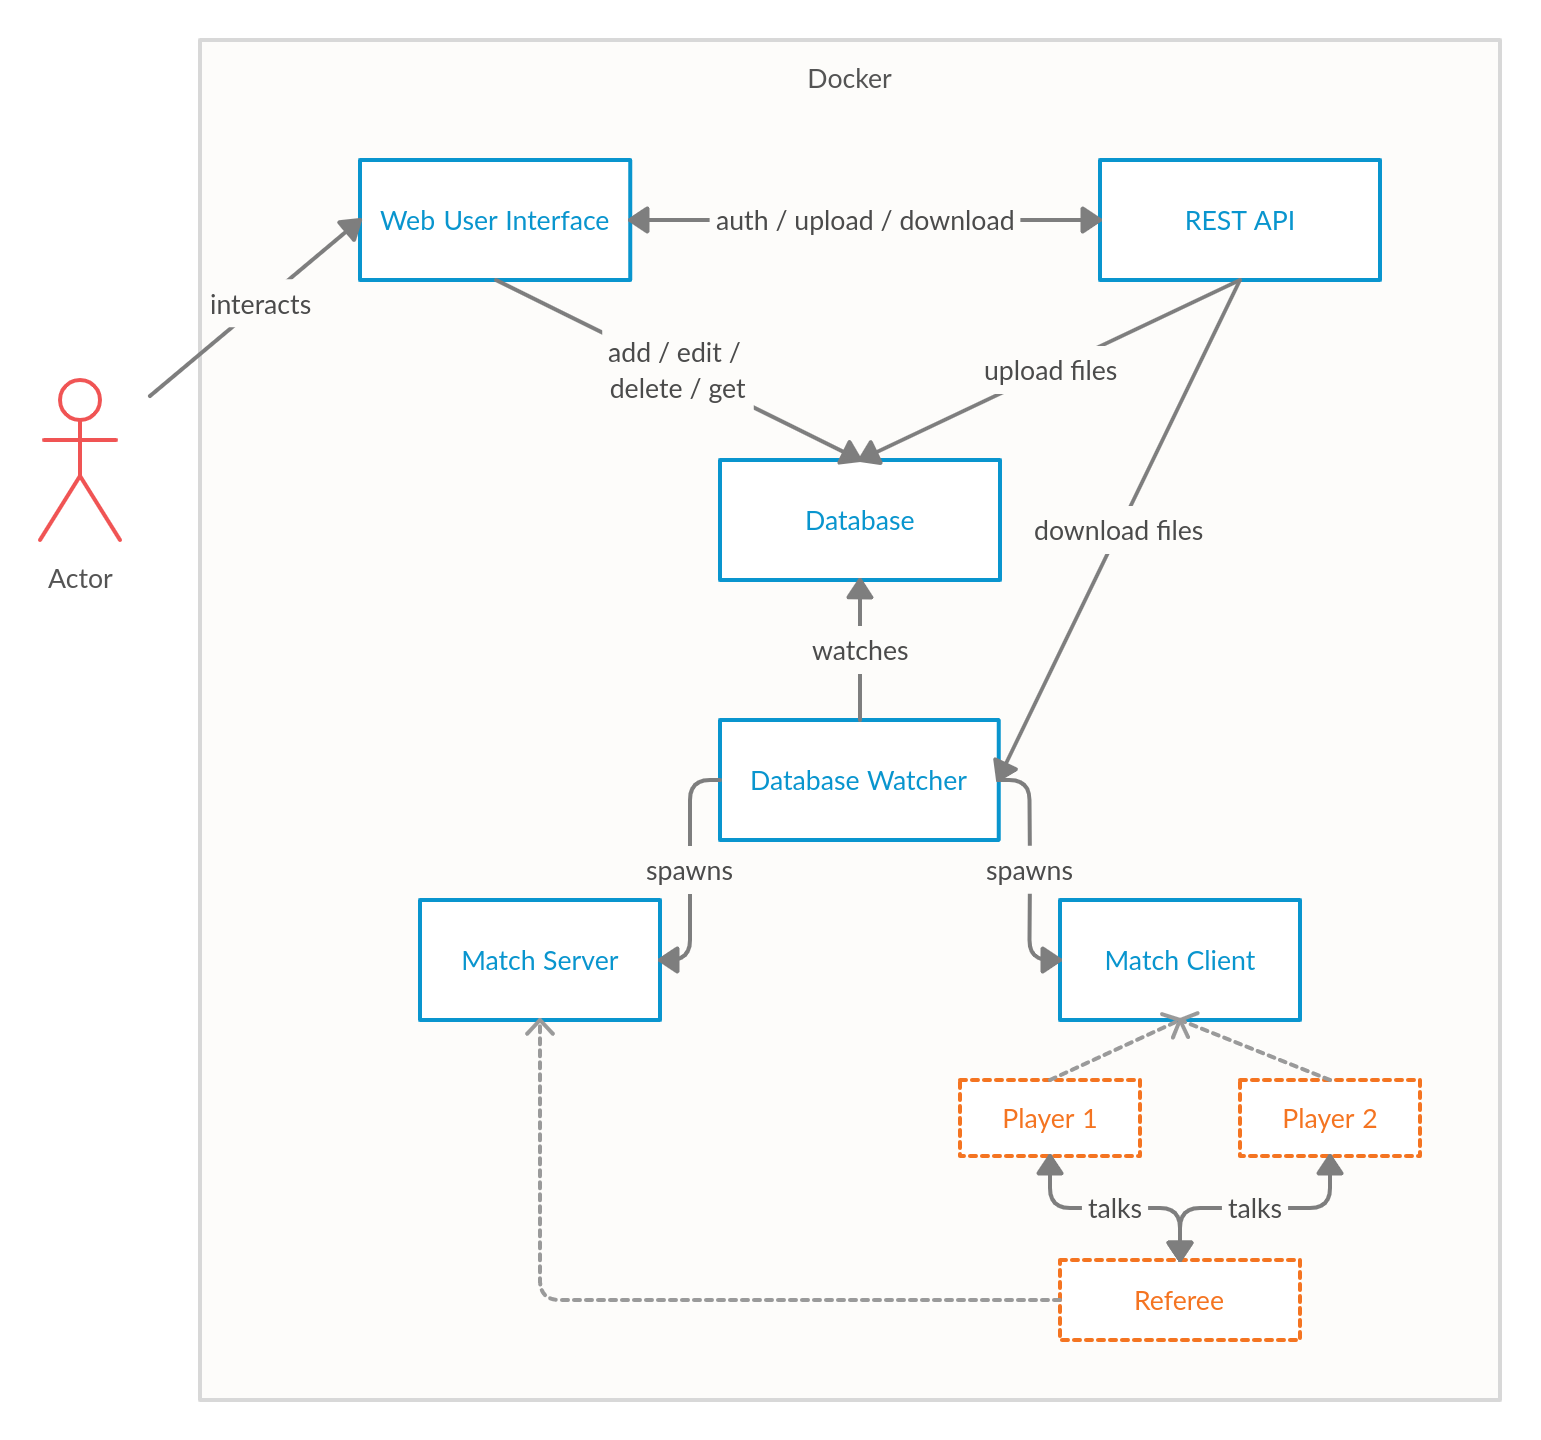
\includegraphics[scale=0.25]{uml-structure.png}
	\caption{UML diagram representing the structure of the FSCTE}
	\label{fig:uml-structure}
\end{figure}

\section{Overview}
\label{sec:impl-overview}

This section serves as an explanation for what can be seen in the UML diagram in
Figure \ref{fig:uml-structure}. \\

The actor represents a user, who can be either an admin or student. This user
only interacts with the web user interface to add players, tournaments and anything
the user desires, provided they have the correct permissions. There is a
difference between a user and a player, where the user is the person who is
currently logged in (student or admin) and the player is an executable that the
user uploads to take part in tournaments. As such, a single user can have many
players. \\

The rectangles with a blue outline represent docker containers and the rectangles
with a dotted orange line represent entities inside the docker containers. The
dotted grey line represents the docker container in which an entity resides.

\section{Web User Interface}
\label{sec:impl-web-interface}

This section serves as an explanation for the purpose of the web user interface
docker container seen in Figure \ref{fig:uml-structure}. \\

The web user interface is designed to be a Single-Page Application (SPA) that
uses components to render specific ``pages'', instead of the traditional way of
rendering complete HTML pages when the user navigates to a different URL route.
This is accomplished by swapping out certain HTML elements with other elements
so that the content of the page changes without having to re-render the elements
that are present in both pages. As such, the performance of a SPA is significantly
better than a traditional web app because of the reduced rendering needed to
display different pages. Vue\footnote{\url{https://vuejs.org/}} was chosen as the
framework to use because it is extremely easy to use and provides support for
creating a SPA. An example of the login screen for the web user interface can be
seen in Figure \ref{fig:login} in the Appendix. \\

The web user interface makes use of cookies to store the session, so that the
user stays logged in even when closing the web user interface browser tab. The
cookies are saved for seven days, meaning that once the cookies expire, the
user has to log in again. Since Vue was chosen as the front-end framework, the
library \texttt{VueCookies}\footnote{\url{https://www.npmjs.com/package/vue-cookies}}
was chosen as the way to store cookies in the web user interface. This library
was easy to use and provided many customizable options, as well as it is
regularly updated. \\

The web user interface consists of different tabs that a user can click to navigate
to different views. The tabs that can be accessed vary depending on the level of
permission of the logged in user, i.e. admins will be able to access more tabs
than students will be able to. However, some tabs are accessible regardless of
if a user is logged in or not. These tabs are the `Tournaments' tab, `Matches'
tab, `Standings' tab and finally the `About' tab. If user logs in as a student,
the user is able to access the `Players' tab as well as all of the tabs
accessible when not logged in. If the user logs in as an admin, the user is able
to access the `Components' tab as well as all of the tabs accessible to a student.
The above tabs will be explained in further detail from section
\ref{sec:impl-tab-tournaments} to \ref{sec:impl-tab-about}.

\subsection{`Tournaments' tab}
\label{sec:impl-tab-tournaments}

The `Tournaments' tab is accessible by a user who is not logged in, a student
and an admin. A screenshot of the page after clicking the tab can be seen in
Figure \ref{fig:all-tourn-student} in the Appendix, when logged in as a student,
and Figure \ref{fig:all-tourn-admin} in the Appendix, when logged in as an
admin.

\subsubsection*{User Not Logged In}

The user is able to view all of the public and private tournaments that are
taking place. An overview of the tournaments is provided where the name of the
tournament, the current status of the tournament (either ``Not Started'',
``Running'' or ``Finished''), the maximum time limit for each move (in milliseconds)
and the number of players currently in the tournament are displayed in a table.
The table uses a live-updating system, meaning that the user does not need to
refresh the page to see any updates to the tournaments, instead the updates are
shown immediately as they happen. \\

The user can click on any entry in the tournaments table to be redirected to
the specific tournament information of the selected tournament. On this page, the
user can see the type of the tournament (either public or private), the status
of the tournament, the maximum time limit per move, the referee used, the scheduler
used and the ranker used. The user can also see the player names of the current
players in the tournament. The ranker, scheduler and referee will be explained
in detail from section \ref{sec:ranker} to \ref{sec:referee}. \\

A table showing the current players participating the selected tournament is
present at the bottom of the selected tournament information page. The user can
see the player names, not the names of the users, of all the players participating
in the selected tournament.

\subsubsection*{User Logged In As A Student}

The user is able to see and do everything described above, as well as being able
to add their own player to a specific public tournament. If the current user has not
uploaded any players, they can select a specific tournament from the table and
they can add a player from within the tournament information page. This will create
a player, link the player to the user and put the player into the selected
tournament. If the user already has uploaded a player, or many players, they will
be presented with a dropdown list of their own players, and the user is then able
to select which player they would like to add to the tournament. \\

If the user has a player participating in the selected tournament, the user can
see the name of their player and remove their player from that tournament if
they wish to do so.

\subsubsection*{User Logged In As An Admin}

The user is able to see and do everything described above, as well as being able
to create a tournament and add students' players to both private and public
tournaments. When creating a new tournament, the user must specify the name of
the tournament, the type (either public or private) and the maximum time per move
(in milliseconds). A check is performed on the name of the tournament, which makes
sure the name is unique. If the name is not unique, the new tournament is rejected
and the user must enter a unique tournament name. \\

If the user selects a specific tournament from the table, the user can add a player
of their own or add a player from a student to the tournament. Only an admin can
add players to a private tournament, but students are able to add their players
to public tournaments. The user can start and stop the tournament as they wish,
as well as edit the information of a specific tournament. When editing the
tournament information, the user can change the name of the tournament, the type
of the tournament, the maximum time limit per move, the referee, the scheduler
and the ranker. A screenshot of the popup displayed when editing a specific
tournament can be seen in Figure \ref{fig:settings-admin}. The user can also
remove any student player from the tournament, as well as being able to delete
the entire tournament if the user wishes.

\subsection{`Matches' tab}
\label{sec:impl-tab-matches}

The `Matches' tab is accessible by a user who is not logged in, a student
and an admin. A screenshot of the page after clicking the tab can be seen in
Figure \ref{fig:matches-student} in the Appendix, when logged in as a student,
and the page is the same for when logged in as an admin or when not logged in.
There is no difference in functionality for matches when not logged in,
logged in as a student or logged in as an admin, because the matches are
automatically generated when a tournament is started. \\

The matches are grouped by their type, meaning that all of the matches played in
a public tournament will be under the `Public' heading and all of the matches
played in a private tournament will be under the `Private' heading. Under each
heading, the matches are organized based on the name of the tournament in which
the matches were played. The matches are displayed in a table, which shows the
ID of the match, the players that participated in the match, the status of the
match and the winner of that match. When clicking on a specific match ID, the user
is redirected to a page that displayed the status of the match, the winner and a
message extracted from the log files. The message gives extra information about
whether an error occurred or, if the match finished successfully, the message will
display the new rating of the two players. There are also buttons at the bottom
of the match information page that allow the user to download each players log
files, as well as the referee log files.

\subsection{`Players' tab}
\label{sec:impl-tab-players}

The `Players' tab is only accessible by a user who is a student or an admin. A
screenshot of the page after clicking the tab can be seen in Figure
\ref{fig:matches-student} in the Appendix, when logged in as a student, and the
page is the same for when logged in as an admin or when not logged in. There is
no difference in functionality for when a user is logged in as a student or an
admin. \\

The players that the logged in user has uploaded is displayed in a table, where
the name of the players are displayed. There is also a button that allows the
user to delete any player they have uploaded, which also removes the player from
any tournaments that it is taking part in. If the user has uploaded players, an
additional section is displayed that shows in which tournaments each player is
participating in. From this additional section, the user can add their player
to another tournament or view the information for the tournaments that the player
already has participated in. A screenshot of the `Players' page can be seen in
Figure \ref{fig:players-student} in the Appendix.

\subsection{`Standings' tab}
\label{sec:impl-tab-standings}

The `Standings' tab is accessible by a user who is not logged in, a student
and an admin. A screenshot of the page after clicking the tab can be seen in
Figure \ref{fig:standings-admin} in the Appendix, when logged in as an admin,
and the page is the same for when logged in as a student or when not logged in.
There is no difference in functionality for the standings when not logged in,
logged in as a student or logged in as an admin, because the standings are
automatically generated when the matches finish. \\

The standings are grouped by their type, meaning that all of the standings in a
public tournament will be under the `Public' heading and all of the standings in
a private tournament will be under the `Private' heading. Under each heading, the
standings are organized based on the name of the tournament. The standings are
displayed in a table, which shows the position of each player relative to the
other players, the name of the players, the number of wins, losses and draws, as
well as the win-loss ratio and the rating for each player.

\subsection{`Components' tab}
\label{sec:impl-tab-components}

The `Components' tab is only accessible by a user who is an admin. A screenshot
of the page after clicking the tab can be seen in Figure \ref{fig:components-admin}
in the Appendix. \\

The components can be seen in a table at the top of the page, where the type of
component (ranker, scheduler or referee) can be seen, as well as the name of the
component and the owner (user who uploaded) of the component. After that table,
there are separate tables for displaying the rankers, schedulers and referees
that the logged in admin user has uploaded. For each of the components that the
admin user has uploaded, the user can change the name of the component or delete
the component. The user can also add a new component by specifying the name of the
component and the file to use as the component. A check is performed on the name
to make sure the name of the component is unique, and if the name is unique then
the component is available to be chosen when selecting the components for a
tournament.

\subsection{`About' tab}
\label{sec:impl-tab-about}

The `About' tab is accessible by a user who is not logged in, a student
and an admin. A screenshot of the page after clicking the tab can be seen in
Figure \ref{fig:about-admin} in the Appendix, when logged in as an admin,
and the page is the same for when logged in as a student or when not logged in.
There is no difference in functionality for the about page when not logged in,
logged in as a student or logged in as an admin, because it is a static page
that doesn't rely on any generated information. \\

The about page describes the types of tournaments that the user can see and
gives an overview of what the ranker, referee and scheduler mean.

\section{REST API}

This section serves as an explanation for the purpose of the REST API docker
container seen in Figure \ref{fig:uml-structure}. \\

The REST API is written in Python 3.7 and Flask\footnote{\url{https://flask.palletsprojects.com/en/1.1.x/}}
because it is very easy to set up. It runs in its own docker container and is
available on port 5000. The API allows for file upload to and download from the
web user interface, as well as providing access points for CAS authentication. \\

File uploading is used for when a user uploads their player using the web user
interface. The file is selected from the user's operating system and uploaded
to the system that is hosting the web user interface. The path to the player
is stored in the database so that the player files can be retrieved when needed.
File downloading is used for when a user wants to download the log files after
a match has finished. The path to the match log is generated by taking the
tournament name and player name of the requested file, then finding the file on
the system hosting the web user interface and finally downloading it to the user's
system. \\

The CAS authentication is used to allow students and lecturers to log into the
web user interface using their Stellenbosch University credentials. When the
user clicks the `SU Login' button on the Login page of the web user interface,
they are redirected to the Single-Sign On page that Stellenbosch uses for
authentication. If the username and password provided is correct, a ticket gets
returned to the REST API, which then gets validated. If the ticket is valid, then
the username is returned to the REST API. If the ticket is not valid, then no
username is returned. After the validation process, the ticket is invalidated so
that it cannot be used again. Once the REST API has the username of the user,
it passes the username back to the web user interface, which checks if the username
is that of a student or admin. It performs this check by looking at the username,
where the username of a student is made up of all numbers and the username of
a lecturer is made up of characters. This user is then added to the database so
that the players associated with the user can be stored in the database. \\

The following endpoints are available for access through the REST API:
\subsubsection*{\texttt{/check}}
\begin{itemize}
	\item \textbf{Usage}: Ensures the REST API is accessible.
	\item \textbf{Methods}: \texttt{GET}
	\item \textbf{Returns}:
	\begin{verbatim}
		{ "message": "Connected successfully" }
	\end{verbatim}
\end{itemize}
\subsubsection*{\texttt{/login}}
\begin{itemize}
	\item \textbf{Usage}: Attempts to log the user in using Stellenbosch
	University credentials.
	\item \textbf{Methods}: \texttt{GET}
	\item \textbf{Returns}:
	\begin{verbatim}
		{
		    "username": <username>,
		    "ticket": <ticket>
		}
	\end{verbatim}
\end{itemize}
\subsubsection*{\texttt{/clear}}
\begin{itemize}
	\item \textbf{Usage}: Logs the Stellenbosch University user out. The logout
	route could not be \texttt{/logout}, since the CAS authentication logout route
	was \texttt{/logout} and various variables needed to be cleared before logging
	the user out.
	\item \textbf{Methods}: \texttt{GET}
	\item \textbf{Returns}: \texttt{None}
\end{itemize}
\subsubsection*{\texttt{/upload/<fileType>/<fileName>}}
\begin{itemize}
	\item \textbf{Usage}: Uploads a \texttt{fileType} called \texttt{fileName}
	to the web user interface local system. The \texttt{fileType} can be either
	a referee, ranker, scheduler or player and the \texttt{fileName} is the name
	of the file to upload.
	\item \textbf{Methods}: \texttt{POST}
	\item \textbf{Returns}:
	\begin{verbatim}
		{ "message" : "File successfully uploaded" }
	\end{verbatim}
\end{itemize}
\subsubsection*{\texttt{/download/<tournamentName>/<fileName>}}
\begin{itemize}
	\item \textbf{Usage}: Downloads the log file called \texttt{fileName} from
	the tournament \texttt{tournamentName}.
	\item \textbf{Methods}: \texttt{GET}
	\item \textbf{Returns}: \texttt{File} object.
\end{itemize}
\subsubsection*{\texttt{/remove/<fileType>/<fileName>}}
\begin{itemize}
	\item \textbf{Usage}: Removes a \texttt{fileType} called \texttt{fileName}
	from the web user interface's local system, if it exists. Mainly used when
	a user deletes a player.
	\item \textbf{Methods}: \texttt{GET}
	\item \textbf{Returns}:
	\begin{verbatim}
		{ "message" : "Successfully deleted file" }
	\end{verbatim}
\end{itemize}

\section{Database}

This section serves as an explanation for the purpose of the database docker
container seen in Figure \ref{fig:uml-structure}. \\

Neo4j\footnote{\url{https://neo4j.com/}} was chosen as the backend database
because the main advantage is the fact that it is a graph database. Graph databases,
such as Neo4j, differ from relational databases, such as SQL, in how they connect
data. Neo4j uses nodes and relationships to connect data, whereas SQL uses
primary and foreign keys. The data that the system uses benefits greatly from
using relationships between nodes to describe the data, since, for example, a user
can have many players (relationship is user to player) that participate in many
tournaments (relationship is user to player to tournament). Such data would require
multiple foreign keys and get very complicated very quickly. \\

Neo4j uses the Cypher query language in order to write queries for the data in
the database. The Cypher query language closely resembles English, making it easy
to write complicated queries and return exactly the data that is needed. Database
drivers were written in both TypeScript, for the web user interface, and Golang,
for the database watcher. The database drivers allowed the web user interface
and the database watcher to add, edit, delete and retrieve data from the
database. An example of the graph database can be seen in Figure \ref{fig:database}
in the Appendix.

\section{Database Watcher}

This section serves as an explanation for the purpose of the database watcher
docker container seen in Figure \ref{fig:uml-structure}. \\

The database watcher was written in Golang because it is a language that handles
concurrency very well, since the first version was released recently, March 2012
\cite{golang}, and has concurrency at its core. Golang is being updated frequently,
with the newest version being released in August 2020. Golang also has multiple
advantages over Java, such as:
\begin{itemize}
	\item Low overhead, since Golang does not use the Java Virtual Machine.
	\item Concurrency is built into the core language and simple to use compared
	to Java threads.
	\item Faster performance when compared to Java.
\end{itemize}
The above advantages are the reason that Golang was chosen over Java for writing
the database watcher. \\

The main role of the database watcher is to watch for any database changes at a
set interval. The main change that the database watcher is looking for is when a
tournament is started or stopped. When this change occurs, the database watcher
retrieves the name of the tournament and retrieves the ranker, scheduler, referee
and players that are participating in that tournament. Information about the
ranker, scheduler and referee is given from section \ref{sec:ranker} to
\ref{sec:referee}.

\subsection{Ranker}
\label{sec:ranker}

The ranker is used to distinguish between the good and bad players by comparing
the rating of the two players, where every player starts on the same rating.
For every win that a player has, their rating increases by some amount and
for every loss that a player has, their rating decreases by some amount. The
amount gained or lost decreases for every match that the player plays, meaning
that eventually the rating will be a true reflection of the skill level of the
player. \\

The ranker needs to be written in Golang so that it can integrate into the database
watcher and the specification for writing the ranker can be found at
\url{https://git.cs.sun.ac.za/20703236/fscte-docs/-/blob/master/guidelines/Ranker.md}.
An example of a ranker that uses the Elo \cite{elo} rating system can be found in
the \texttt{mock-data} directory in the root of the FSCTE repository and it is
called \texttt{EloRanker.go}.

\subsection{Scheduler}
\label{sec:scheduler}

The scheduler is used to schedule matches between two players that play against
each other in order to see who is the better player. After every player
has played against every other player in the tournament, the overall win-loss
ratio for that tournament can be calculated, which can then be used to
distinguish between good, average and bad players. The win-loss ratio and the
rating system can be used in conjunction to organize fair matches between players
are of a similar skill level. \\

The scheduler needs to be written in Golang so that it can integrate into the
database watcher and the specification for writing the scheduler can be found at
\url{https://git.cs.sun.ac.za/20703236/fscte-docs/-/blob/master/guidelines/Scheduler.md}
An example of a scheduler that uses a round-robin strategy to organize matches
between players can be found in the \texttt{mock-data} directory in the root of
the FSCTE repository and it is called \texttt{RoundRobin.go}.

\subsection{Referee}
\label{sec:referee}

The referee is used to monitor the moves that the two players make in a match and
check if any player makes an invalid move or times out. One player sends a
move to the referee, which then checks if the move is valid and only sends
the move to the other player if the move made is valid. If the move made is
invalid, or the player times out, the match will be forfeit and the last player
to send a valid move becomes the winner. \\

The referee needs to be a \texttt{JAR} file that is compatible with a game type
supported by the Ingenious
Framework\footnote{\url{https://bitbucket.org/skroon/ingenious-framework/src/master/}}.
An example of a referee for the Othello game is provided in the \texttt{mock-data}
directory in the root of the FSCTE repository and it is called \texttt{OthelloReferee.jar}.

\subsection{Match Server}

The match server docker container is started when a new tournament is started,
which starts the Java server using the referee that the tournament uses. The match
server lasts for only a single match and the log file from the perspective of the
referee is stored on the FSCTE local system. A path to the match log file is stored
in the database so that the referee log file can be downloaded from the web user
interface at a later stage.

\subsection{Match Client}

The match client docker container is started after the match server docker container
is started, and is used to create the lobby for two of the players in the tournament
as well as play out the match between the players. The way the two players are
selected is defined by the scheduler that is used for the tournament and the
rating update after the match has concluded is defined by the ranker used in the
tournament. \\

The match lobby is created in the match client docker container and then the
players are copied from the FSCTE local system into the match client docker
container. The players are then connected to the match server and play against
each other by sending their moves to the referee, which verifies if the moves are
valid and if they are valid, then the referee sends the move to the other player.
This process continues until either a player sends an invalid move or the game
is played out until completion. The log files of each player are stored and the
path to the log files are added to the database so that each player log file can
be downloaded at a later stage using the web user interface.

\section{Repository}

The code is hosted on GitLab as a private repository and can be found at
\url{https://git.cs.sun.ac.za/20703236/fscte}. The instructions on how to start
all of the docker containers is in the README, which is accessible at
\url{https://git.cs.sun.ac.za/20703236/fscte/-/blob/master/README.md}. All of
the files present in the repository take up 36 Megabytes of space and consist
of $11 652$ lines of code written from scratch. Vue makes up 53.2\% of the code
base, with Go making up 22\%, TypeScript making up 19.4\%, Shell making up 4.1\%,
Python making up 0.9\% and the rest of the languages making up 0.4\% of the code
base.

\chapter{Testing}
\label{chap:testing}

This chapter covers the testing that has been done on the FSCTE to ensure that
every unit of the system works as intended, and also allows future developers to
see if any change they make breaks existing functionality or not. The individual
units of the system need to be tested, but the integration between the units and
the system as a whole also needs to be tested. The unit testing will be discussed
in section \ref{sec:unit-test} and the integration testing will be discussed in
section \ref{sec:integ-test}.

\section{Unit Testing}
\label{sec:unit-test}

This section describes the unit testing that is performed on each component of
the FSCTE system.

\subsection{Web User Interface}

The web user interface was tested manually by going through the entire web user
interface. The login was tested using the following methods:
\begin{itemize}
	\item \textbf{Admin username with wrong password}: The web user interface
	rejected the login attempt and displayed a popup message saying ``Incorrect
	username and password combination.'' This is the expected result.
	\item \textbf{Admin username with correct password}: The web user interface
	accepted the login attempt and redirects to the \texttt{/dashboard} page.
	This is the expected result.
	\item \textbf{Student login using incorrect SU credentials}: The web user
	interface redirects to the Stellenbosch University Single-Sign On page,
	where the incorrect credentials are inputted. The Single-Sign On page rejects
	the login attempt and displays a message stating: ``Sign-on failed. Username
	or password is incorrect.'' This is the expected result.
	\item \textbf{Student login using correct SU credentials}: The web user
	interface redirects to the Stellenbosch University Single-Sign On page,
	where the correct credentials are inputted. The Single-Sign On page accepts
	the login attempt and redirects to the \texttt{/dashboard} page. This is the
	expected result.
\end{itemize}
The tournaments page was tested by adding a tournament manually into the database
and checking if the tournament was updated in the table of tournaments. For all
the various tournaments that were manually added, the tournaments appeared
immediately in the table of tournament present. \\

The matches page was tested by starting various tournaments at the same time,
which started the match scheduling in the database watcher. After each match
had completed, the status in the web user interface was updated, as expected,
with the result of the match. When an error occurred, causing the match to
fail, the winner was reported to be ``Invalid'', which was expected. A detailed
log of what caused the match to fail was accessible by clicking on the match
in the matches table. When the match completed successfully, with no players
failing or running out of time, the winner was reported. The winner was verified
by looking at the referee log file, and of all the matches that completed
successfully, the winner was reported correctly. Downloading the log files was
tested by clicking on the specific log files and checking the contents of the
file, to make sure that the match file downloaded was indeed the correct match
file. In all cases, the correct match log files were downloaded. \\

The players page was tested by adding a player and checking if the table displaying
the players updated with the correct player name. The added players were also tested
by adding them to a tournament and then starting the tournament, thus creating
matches in which the players would play each other. The players were successfully
added to all the tournaments and successfully played all the matches, resulting
in one of the players being the best with an almost flawless win-loss ratio.
This was deemed to be working as intended, since after playing multiple matches
against various opponents, there will always be at least one player that is the
best. \\

The standings page was tested by starting tournaments and waiting for all of
the matches to finish. Once the matches have finished, the results of the matches
were checked. Whenever a player wins against another player, their rating should
increase and if they lose against another player, their rating should decrease.
If the match results end in a draw, neither player's rating increases or decreases.
This result was checked against the standings table, to see if the standings
updated after a match was played. It was found that the standings were automatically
updated as soon as the match concluded, and the winner was the same as the winner
found in the log file. \\

The components page was tested by adding and removing components and checking if
they were updated in the components table. Only the admin user is able to test
the components, since the admin is the only user that has access to the components
page. It was seen that adding and removing components from the database added
and removed the components from the web user interface as well, which is the
expected result. \\

There was no need to test the about page, since it is a static page that does
not have any generated data.

\subsection{Database}

The database was tested using Python and the Neo4j pip package. Various methods
were tested to see if, after adding or deleting nodes from the database, the
backend database would change. After multiple tournaments were added and removed,
as well as adding players and removing players, the database did indeed change
and the actions were reflected. \\

The database was also tested using the Golang test suite, which is built into
the core language. Some small errors were discovered when testing using the
Golang test suite, which have now since been fixed and all test cases pass.

\section{Integration Testing}
\label{sec:integ-test}

This section describes the integration testing performed on the FSCTE system.

\subsection{Tournaments running concurrently}

It is a requirements that the tournaments are able to be run concurrently, so
that no tournament needs to wait for another tournament to finish before another
can start. Golang was useful here because of the built-in concurrency it brings
and the concurrent tournaments were tested by starting multiple tournaments at
the same time. It was seen that the matches were scheduled independently of one
another and all of the matches in each scheduled tournament finished. \\

The match results were checked by downloading the log files and checking that the
result obtained from the log file is the same as the reported result by the match
table. For all the matches that were played, the log files and match table results
were the exact same, hence the concurrent tournaments worked as expected.

\chapter{Future Work}
\label{chap:future}

This chapter covers the future work that could be implemented in the Fail-Safe
Cloud Tournament Engine (FSCTE) to extend the current functionality. The
conclusion will be provided in section \ref{chap:conclusion}.

\section{Kubernetes}

Kubernetes\footnote{\url{https://kubernetes.io/}} can be used to manage the docker
containers, so that if a container crashes, another instance of that container
can be redeployed without hesitation. Due to time constraints, it was not feasible
to add Kubernetes to the current FSCTE.

\section{Other Game Types}

In the current FSCTE implementation, only the \texttt{Othello} game is supported.
Supporting other game types will allow the FSCTE to be more abstract and versatile.
Due to time constraints, it was not feasible to attempt to support other types
of games.

\chapter{Conclusion}
\label{chap:conclusion}

The main requirements of the FSCTE that needed to be satisfied were:
\begin{itemize}
	\item have effective error handling
	\item have effective debugging facilities
	\item scale with tournaments and players
	\item have a logical, clean and maintainable code base
	\item have a more user-friendly web user interface
\end{itemize}
All of the above requirements were satisfied. The error handling requirement
was satisfied by making sure that at any point where an error could occur, it
was decided if the error was serious or not. If the error was serious, then an
error message would be displayed and the component that caused the error would
be stopped. If the error was not serious, then an error message would be displayed,
but nothing would happen to the component that caused the error. \\

The effective debugging facilities requirement was satisfied by logging all
information that happens inside each docker container, so that if some error
occurs, the user can look in the docker logs to see at which stage the error
occurred. This allows the user to know exactly what was going on before the
error occurred so that the user can pinpoint the issue and fix the problem. \\

The tournaments and player scaling requirement was satisfied by writing the
code base in such a way that it performs very well for any number of tournaments
and players. Golang was mainly used to allow scaling to be possible through the
use of concurrent threads running different tasks at the same time. \\

The maintainable code base requirement was satisfied by providing extensive
documentation throughout the code base, so that anyone who reads the code base
can understand what is going on without any issue. \\

The user-friendly web user interface requirement was satisfied by ensuring that
the user can navigate to any page or get any information they want in a maximum
of two mouse clicks. A lot of time was spent making sure that the web user
interface looked clean and visually appealing, as well as easy to use. \\

Working on the FSCTE for the past year has been a great challenge, but also a
great reward. Initially, it was tough to understand what was going on in the CTE
because of the lack of documentation and confusing way that some sections were
implemented. After understanding the previous work, the toughest challenge was
getting the players to play a match and communicate their results to the web
user interface. However, it was a fun and informative experience.

\chapter{Appendix}

\section{Web User Interface}

The images from Figure \ref{fig:login} to \ref{fig:about-admin} are screenshots
from the web user interface that the admins and students will interact with.
\vspace{0.4cm}

\begin{figure}[H]
	\centering
	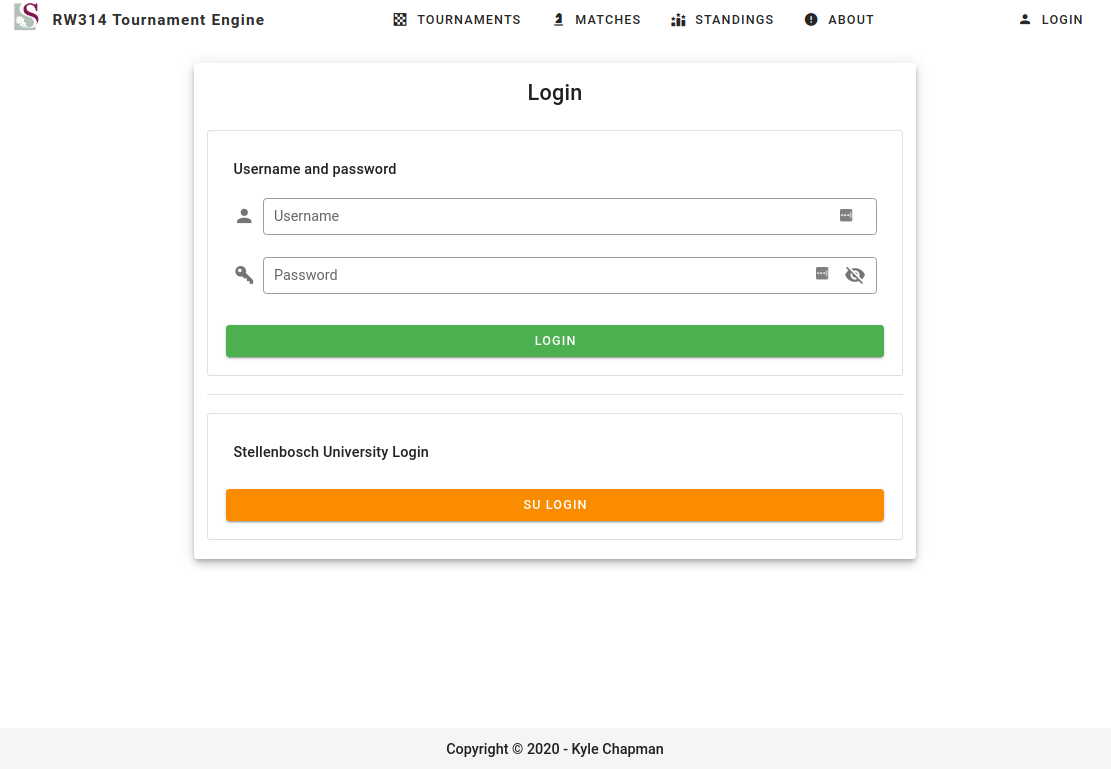
\includegraphics[scale=0.41]{login.png}
	\caption{Login page}
	\label{fig:login}
\end{figure}
\begin{figure}[H]
	\centering
	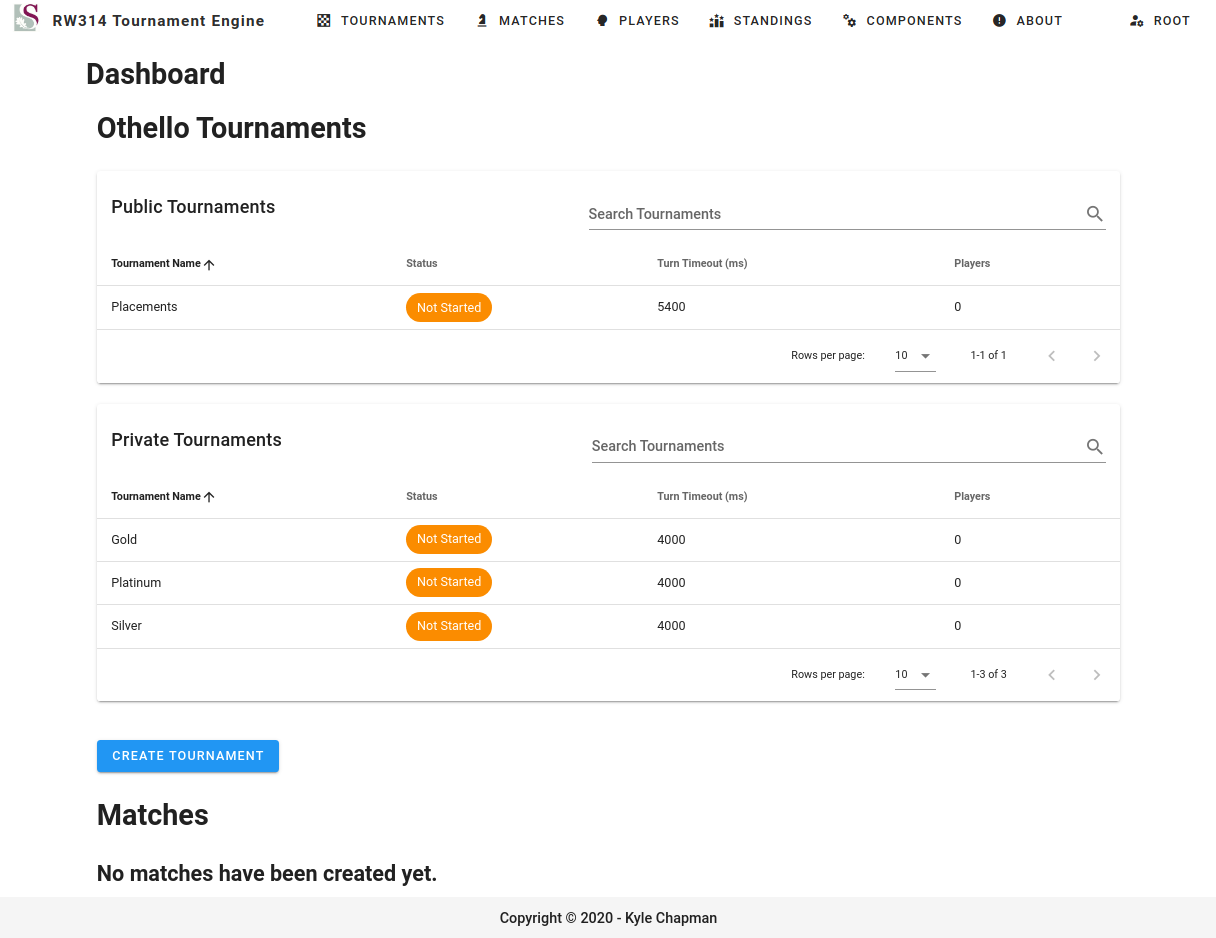
\includegraphics[scale=0.37]{dashboard-admin.png}
	\caption{Dashboard after logging in as admin}
	\label{fig:dashboard-admin}
\end{figure}
\begin{figure}[H]
	\centering
	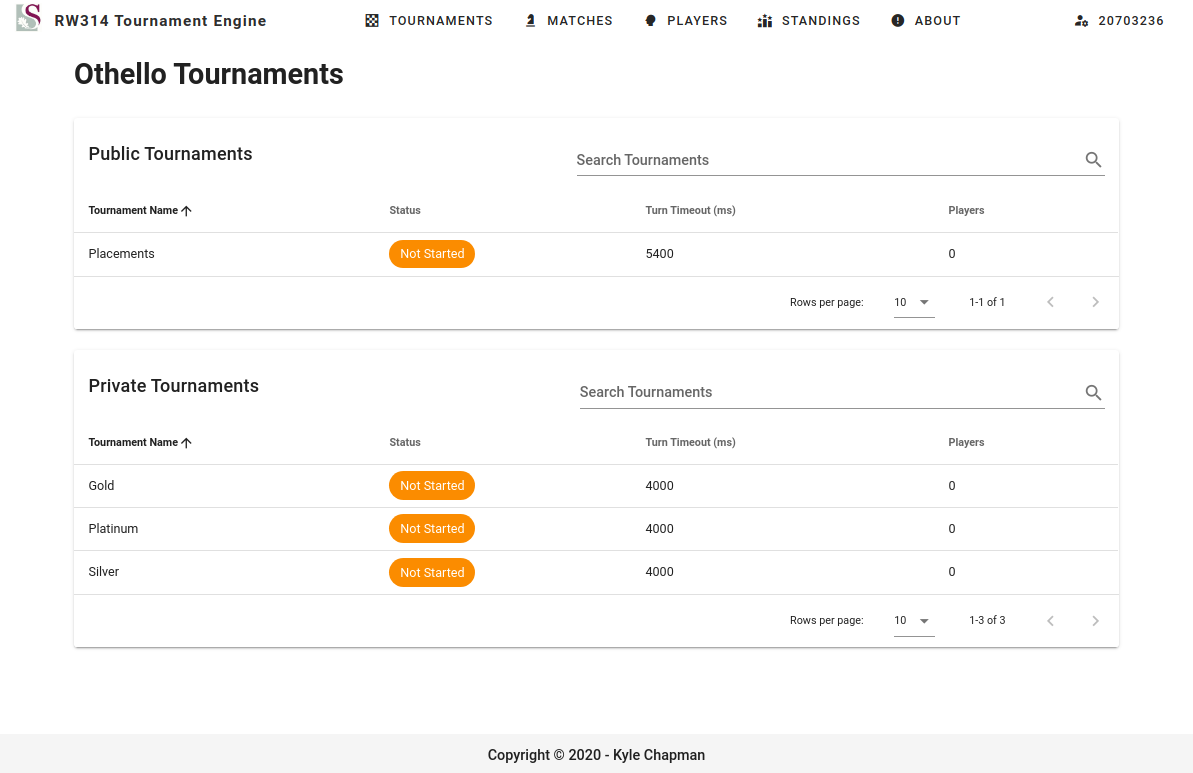
\includegraphics[scale=0.33]{all-tournaments-student.png}
	\caption{`Tournaments' tab when logged in as a student}
	\label{fig:all-tourn-student}
\end{figure}
\begin{figure}[H]
	\centering
	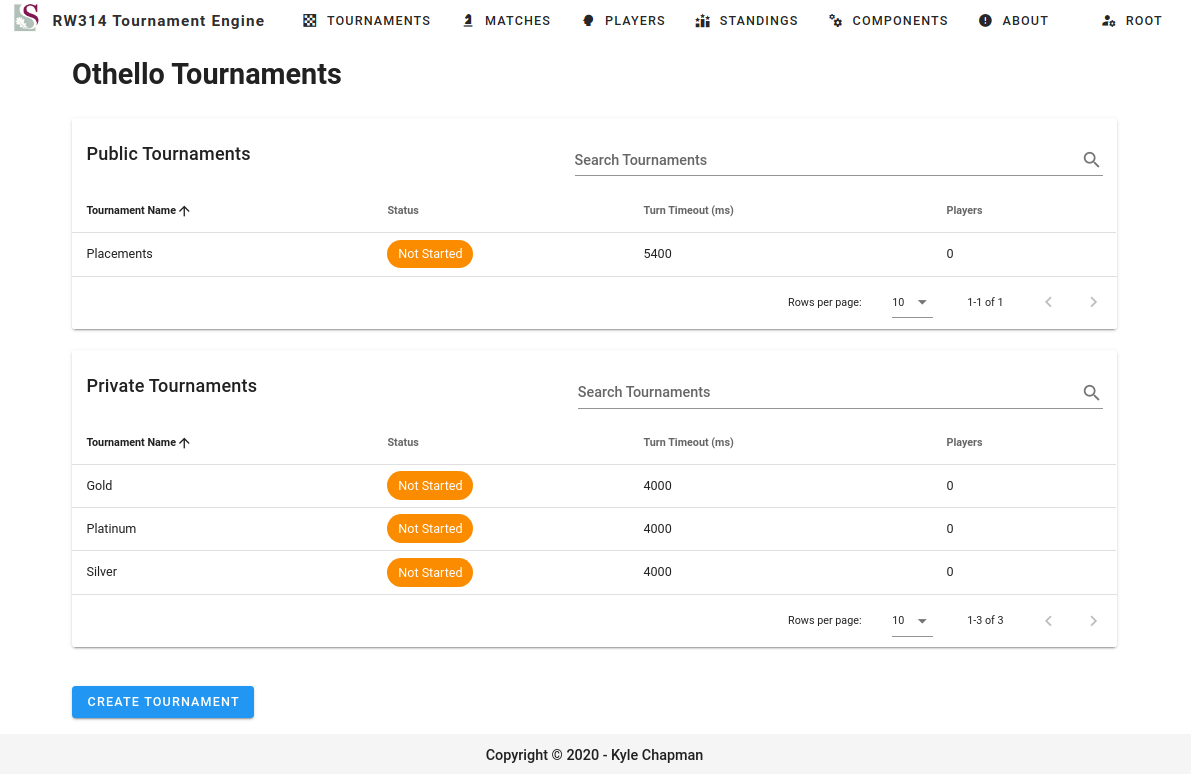
\includegraphics[scale=0.33]{all-tournaments-admin.png}
	\caption{`Tournaments' tab when logged in as an admin}
	\label{fig:all-tourn-admin}
\end{figure}
\begin{figure}[H]
	\centering
	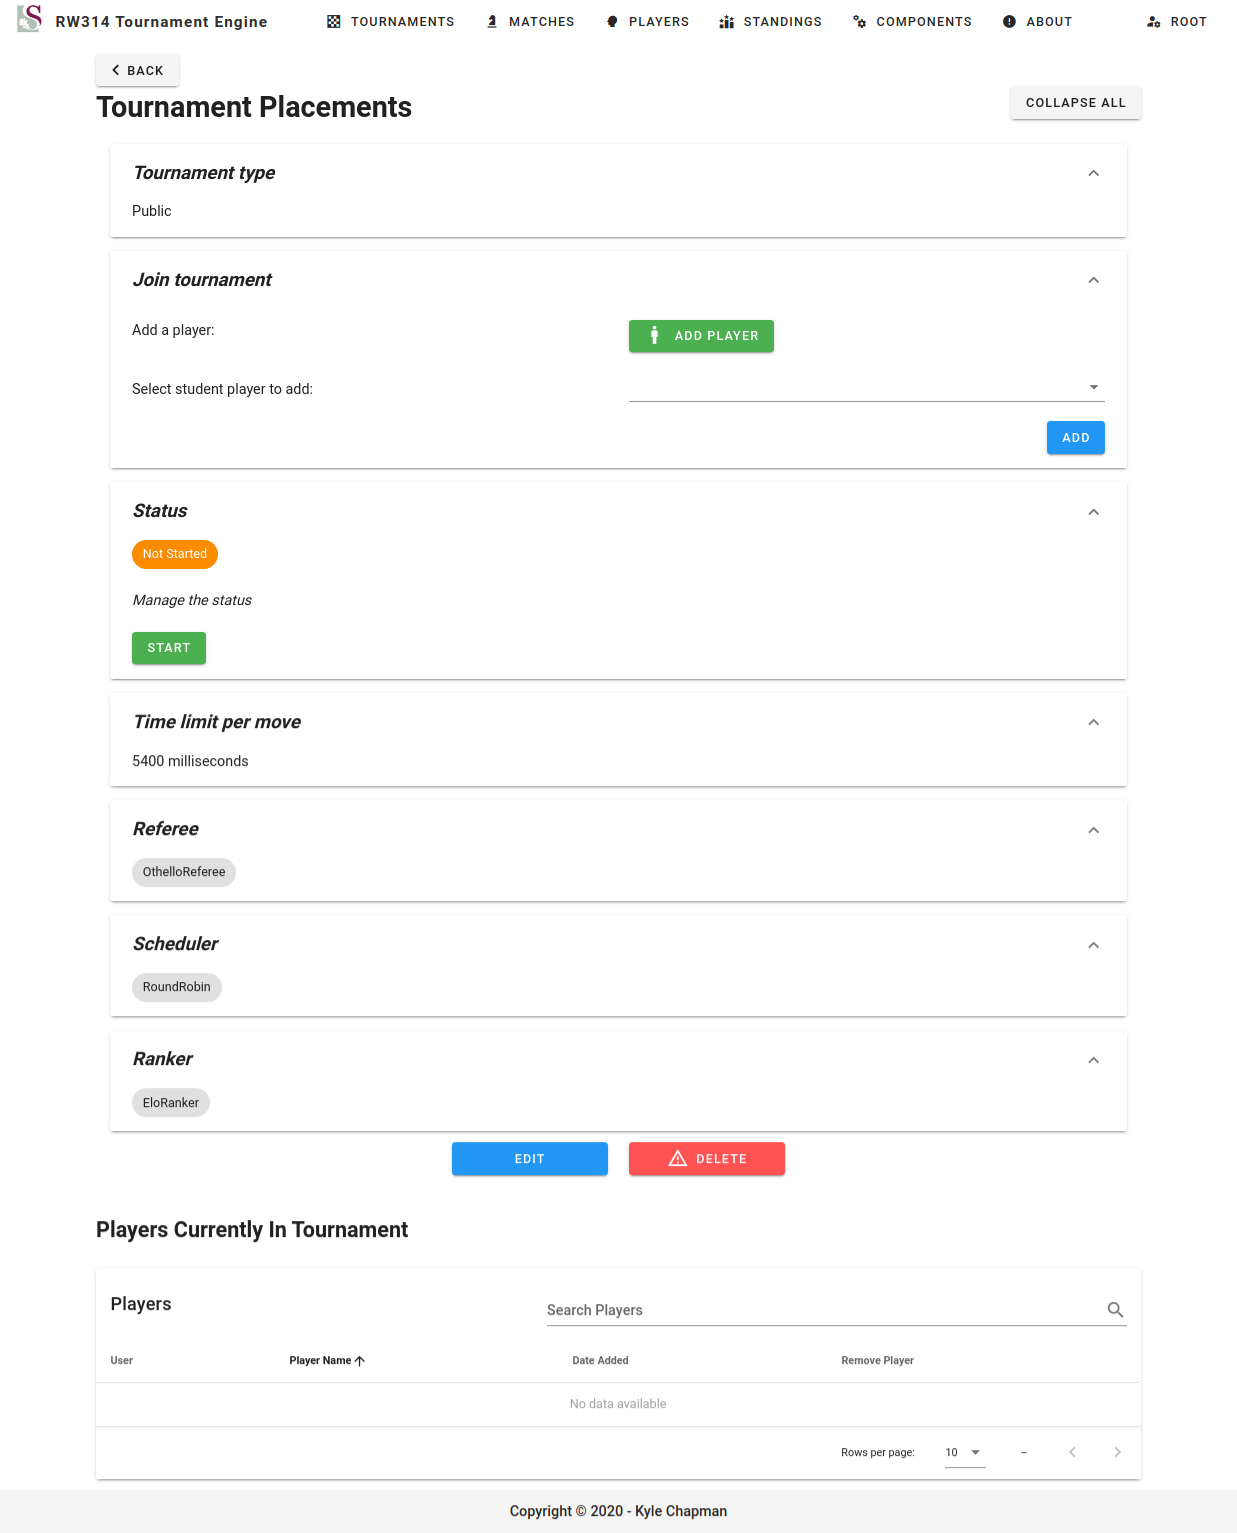
\includegraphics[scale=0.37]{tournaments-admin.png}
	\caption{Page describing the tournament `Placements'}
	\label{fig:tourn-placements}
\end{figure}
\begin{figure}[H]
	\centering
	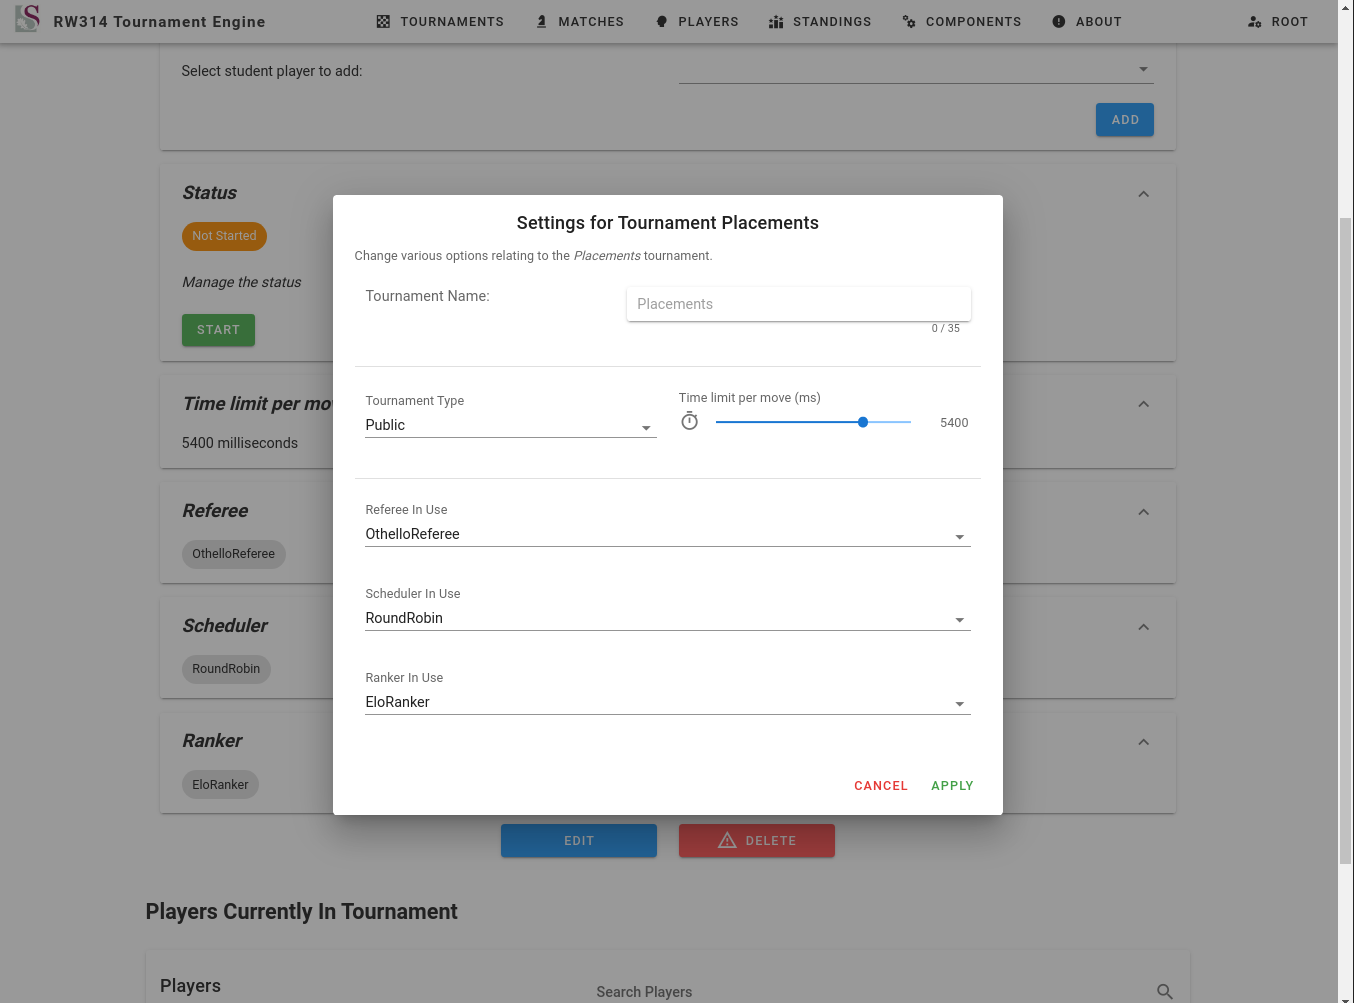
\includegraphics[scale=0.33]{settings-admin.png}
	\caption{Settings popup for the tournament `Placements' when the logged in user is an admin}
	\label{fig:settings-admin}
\end{figure}
\begin{figure}[H]
	\centering
	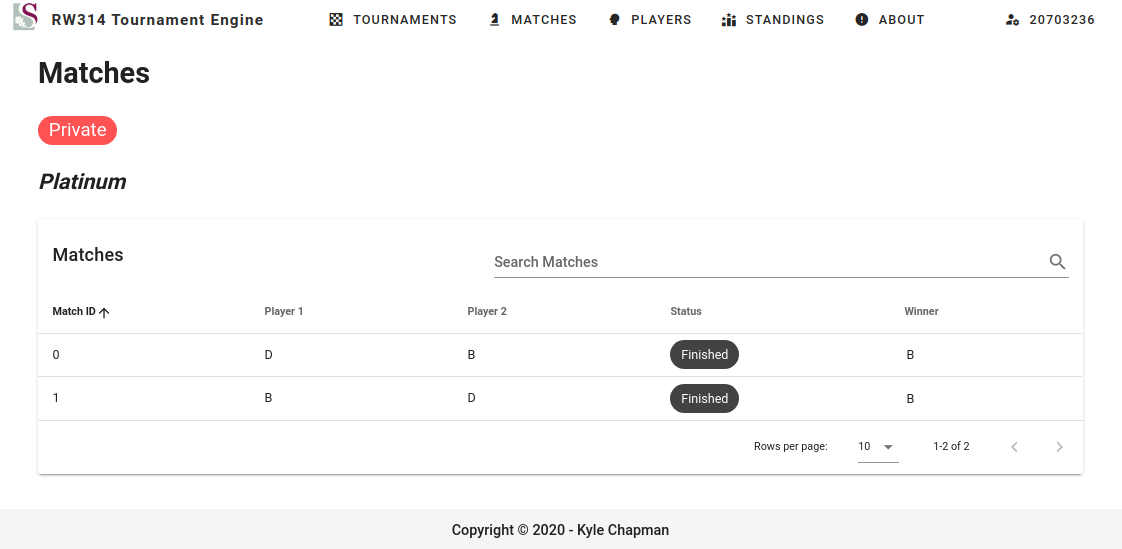
\includegraphics[scale=0.38]{matches-student.png}
	\caption{`Matches' tab when logged in as a student}
	\label{fig:matches-student}
\end{figure}
\begin{figure}[H]
	\centering
	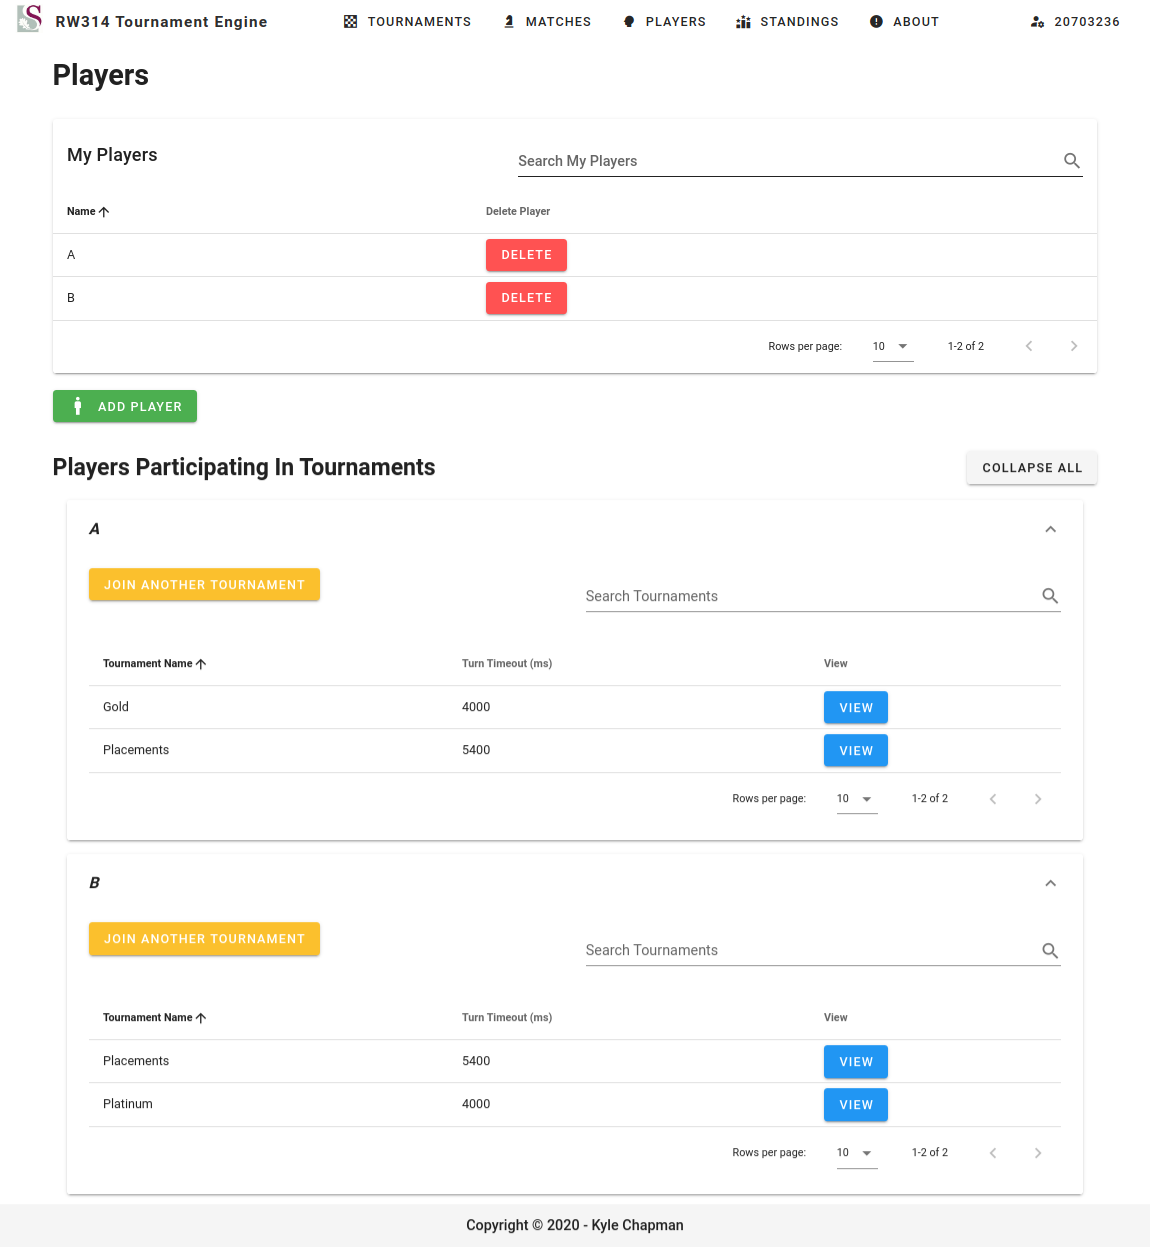
\includegraphics[scale=0.37]{players-student.png}
	\caption{`Players' tab when logged in as a student}
	\label{fig:players-student}
\end{figure}
\begin{figure}[H]
	\centering
	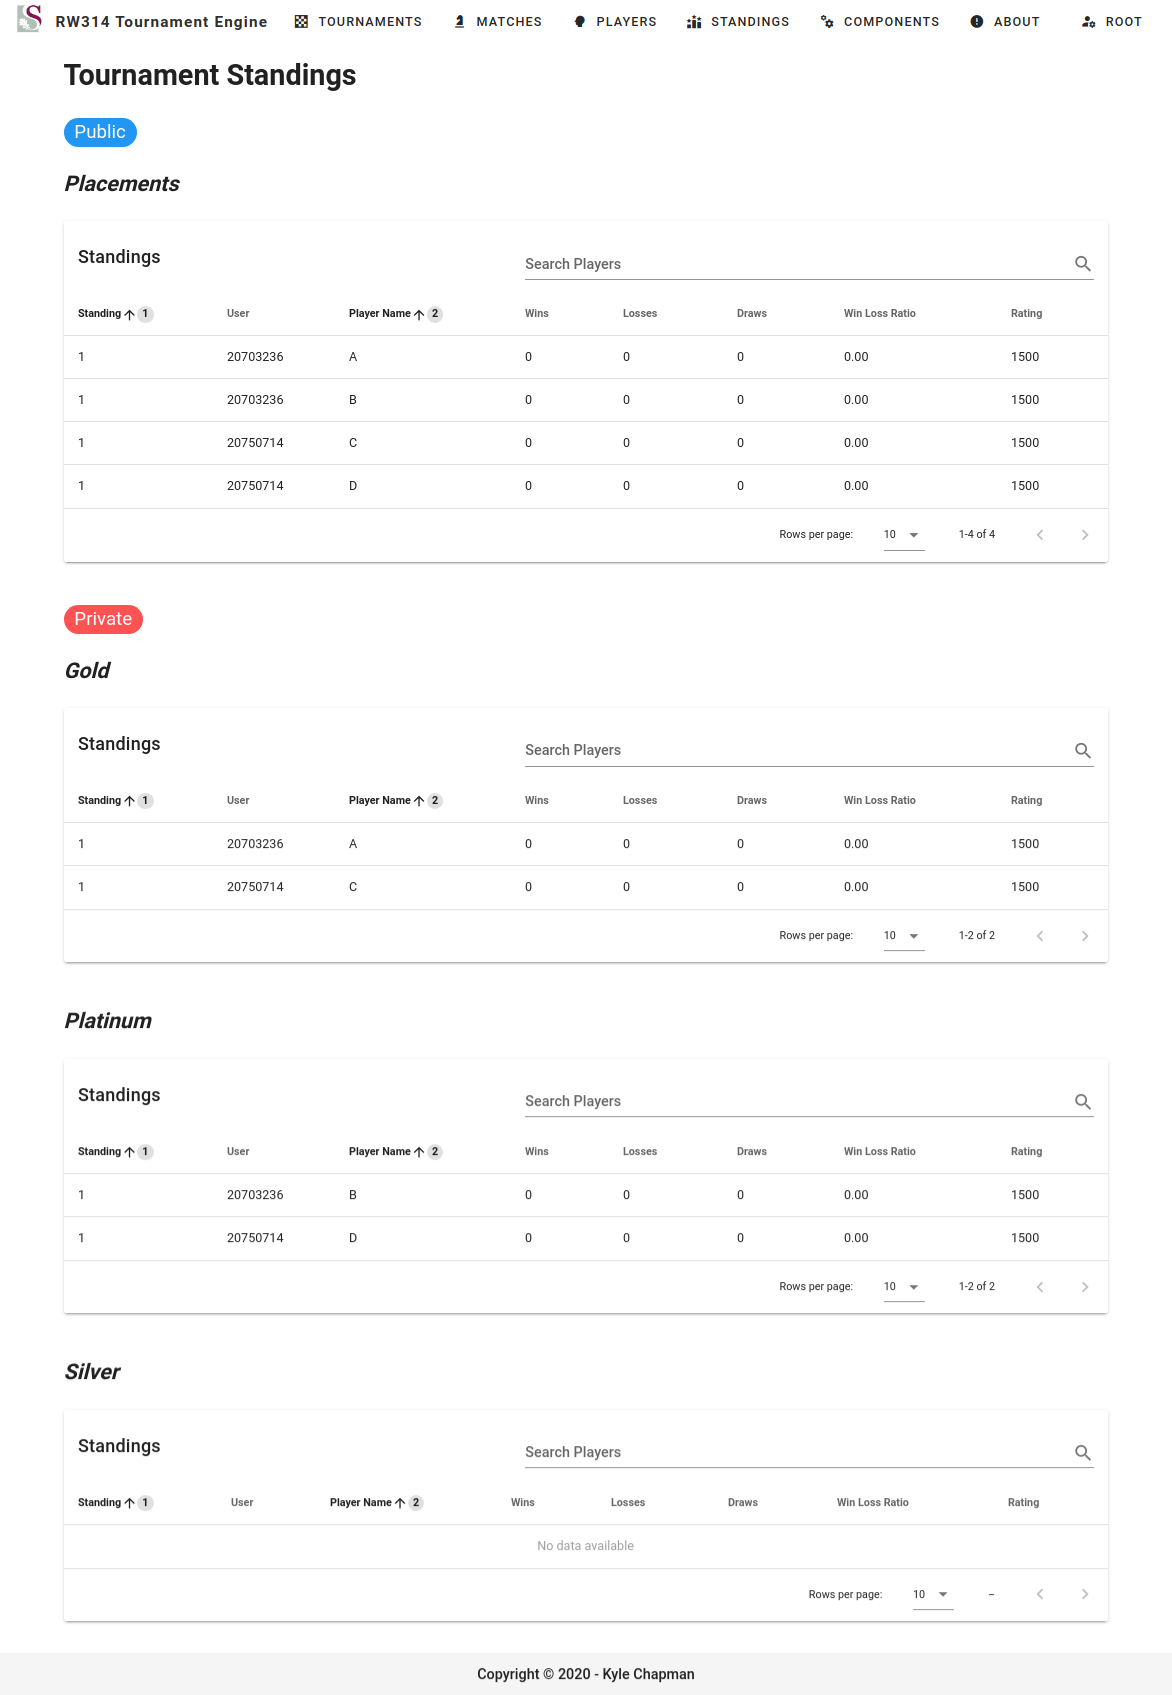
\includegraphics[scale=0.33]{standings-admin.png}
	\caption{`Standings' tab when logged in as an admin}
	\label{fig:standings-admin}
\end{figure}
\begin{figure}[H]
	\centering
	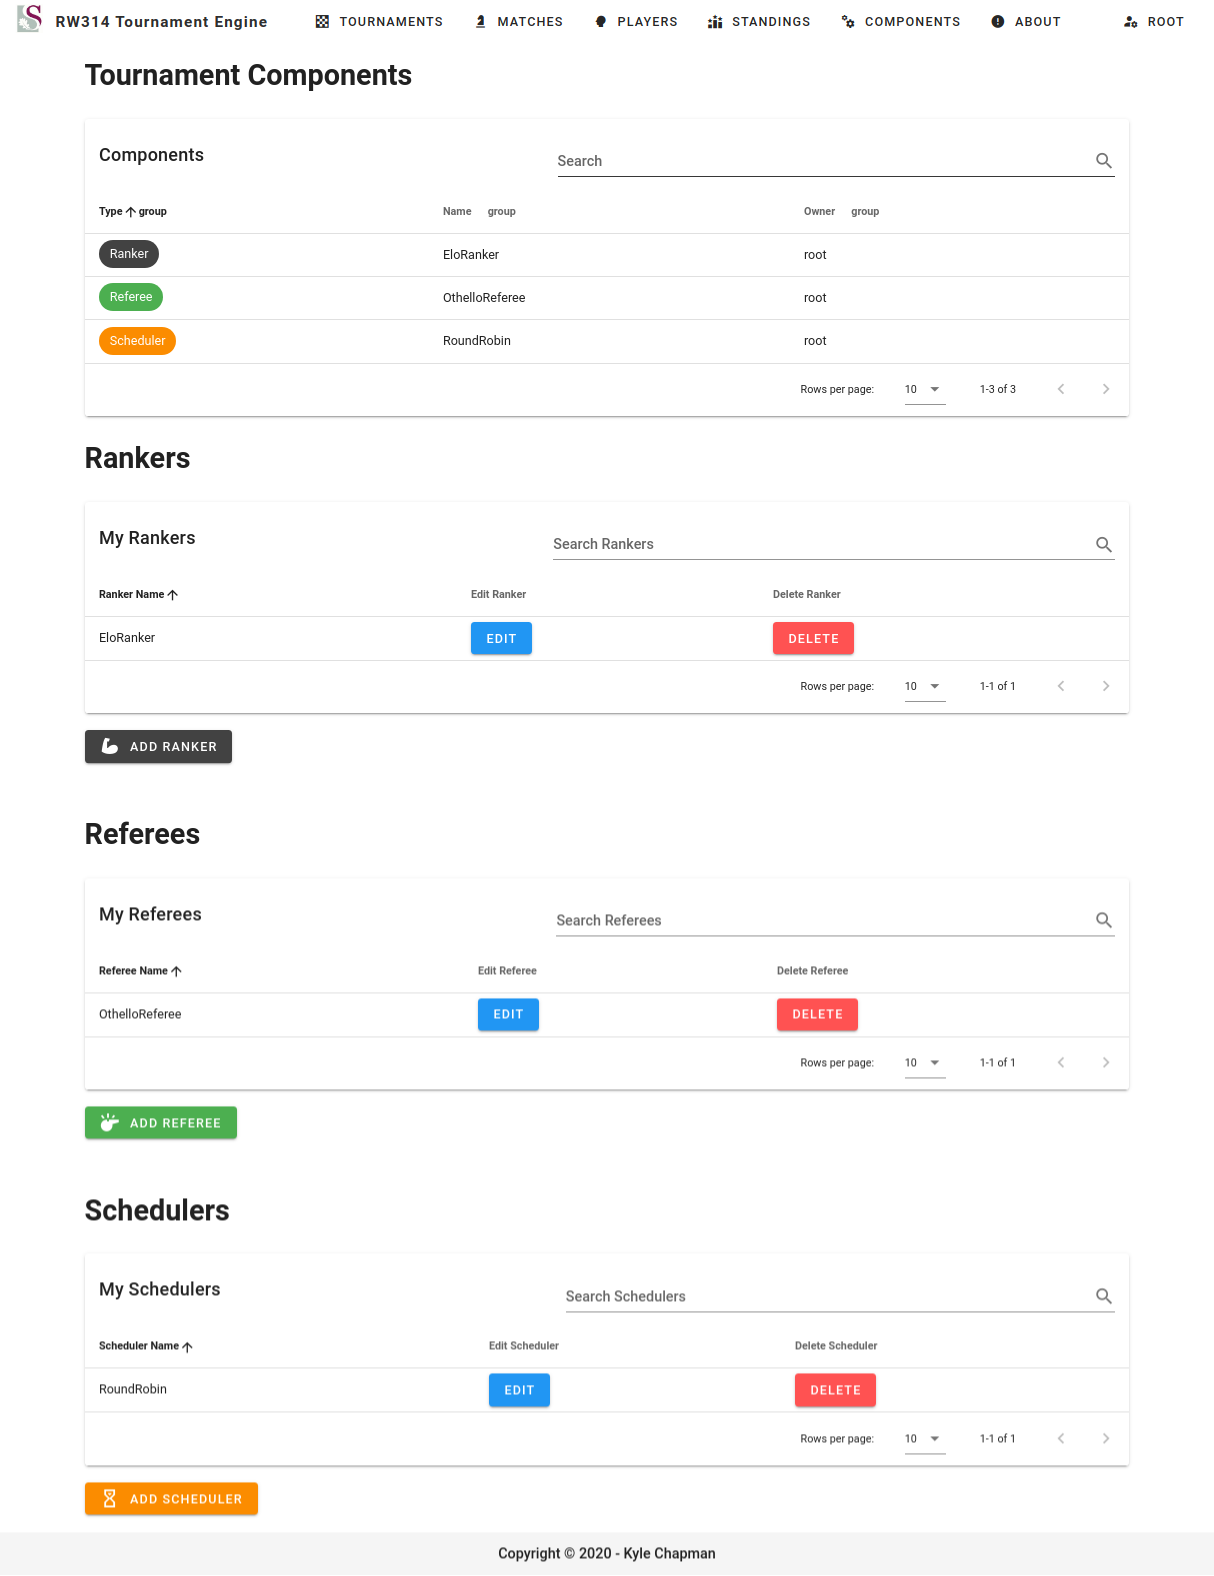
\includegraphics[scale=0.35]{components-admin.png}
	\caption{`Components' tab when logged in as an admin}
	\label{fig:components-admin}
\end{figure}
\begin{figure}[H]
	\centering
	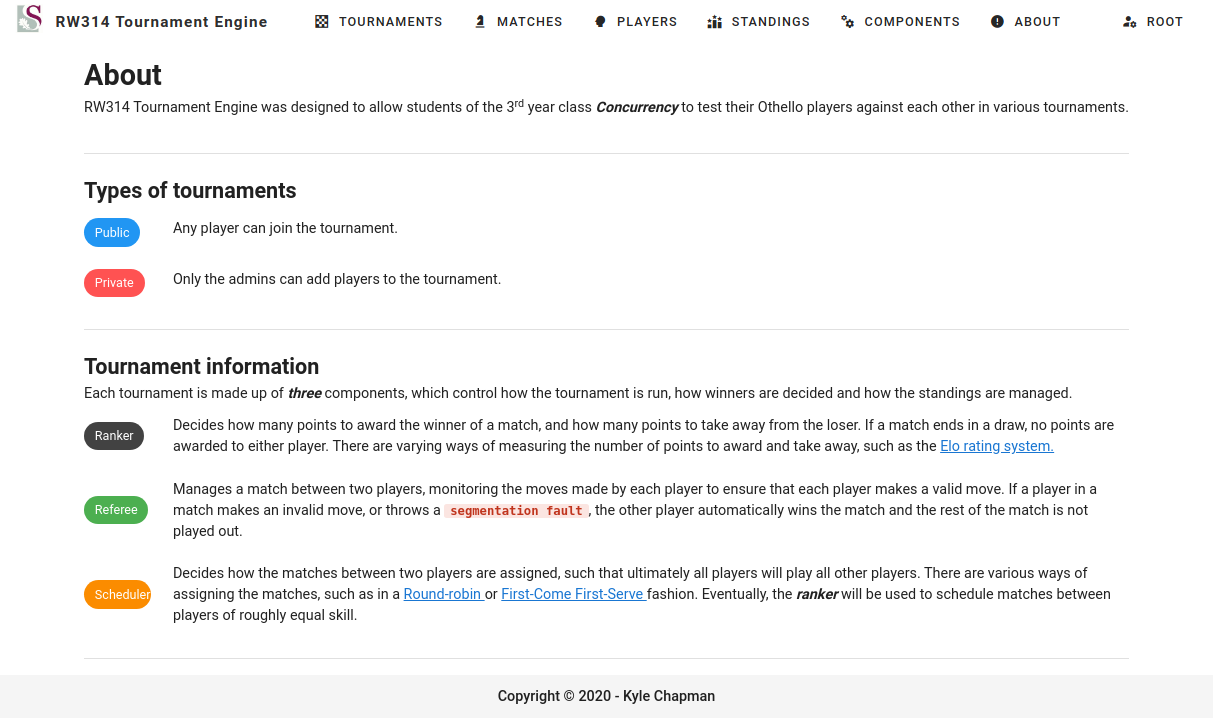
\includegraphics[scale=0.37]{about-admin.png}
	\caption{About page}
	\label{fig:about-admin}
\end{figure}

\section{Database}

\begin{figure}[H]
	\centering
	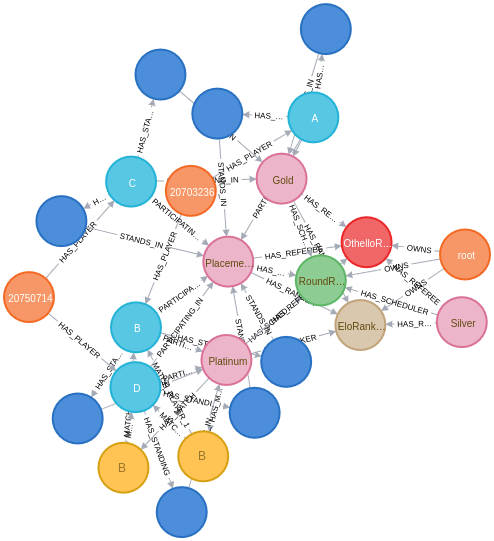
\includegraphics[scale=0.55]{graph-ex.png}
	\caption{An example of the data connected in the Neo4j database}
	\label{fig:database}
\end{figure}

\printbibliography

\end{document}
